\documentclass[a4paper,11pt,titlepage]{article}

\usepackage{ucs}
\usepackage[german,ngerman]{babel}
\usepackage{fontenc}
\usepackage[pdftex]{graphicx}
\usepackage[pdftex]{hyperref}
\usepackage{listings}
\usepackage{xcolor}

\definecolor{codegreen}{rgb}{0,0.6,0}
\definecolor{codegray}{rgb}{0.5,0.5,0.5}
\definecolor{codepurple}{rgb}{0.58,0,0.82}
\definecolor{backcolour}{rgb}{0.95,0.95,0.95} % Very light gray


\lstdefinestyle{mystyle}{
    backgroundcolor=\color{backcolour},
    commentstyle=\color{codegreen},
    keywordstyle=\color{magenta},
    numberstyle=\tiny\color{codegray},
    stringstyle=\color{codepurple},
    basicstyle=\ttfamily\footnotesize,
    breakatwhitespace=false,
    breaklines=true,
    captionpos=b,
    keepspaces=true,
    numbers=left,
    numbersep=5pt,
    showspaces=false,
    showstringspaces=false,
    showtabs=false,
    tabsize=2,
    frame=tlbr, % adds a frame around the code
    framesep=5pt, % padding thickness
    framerule=0pt % frame thickness
}

\lstset{style=mystyle}
\begin{document}

    \title{Einf\"uhrung in die Informatik\\
    Ausarbeitung \"Ubung 4}


    \author{Tim Zolleis}

    \date{\today}

    \maketitle{\thispagestyle{plain}}


    \section{Aufgabe 1 - Apache Webserver}

    \subsection{Problem}
    Eine einfache HTML Website soll mit dem Apache-Webserver gehosted werden. Daf"ur muss:
    \begin{enumerate}
        \item Das Paket des Webservers installiert werden
        \item Die Konfiguration des Webservers angepasst werden, sodass dieser auf einem Port gr"oßer 1024 l"auft
        \item Die Website in das Verzeichnis des Webservers kopiert werden
        \item Eine entsprechende Konfiguration (hier ein Virtualhost) erstellt werden, die das Verzeichnis (bzw. die index.html) der erstellten Website referenziert
    \end{enumerate}

    \subsection{konkrete L"osung}

    \subsubsection{Installation}
    Zun"achst muss der Apache-Webserver installiert werden. Dies kann entweder direkt (\textbf{apt install apache2}) oder mit Docker realisiert werden.

    \subsubsection{Apache-Konfiguration}
    Um den Port, unter dem Apache l"auft zu "andern, m"ussen entsprechende Konfigurationsdateien im Konfigurationsverzeichnis von Apache (unter ubuntu \textbf{/etc/apache2}) bearbeitet werden.
    Konkret ist hier die \textbf{ports.conf} Datei interessant. Die Listen-Direktive spezifiert den Port. Diese k"onnen wir z.B auf \textbf{8080} setzen.

    \begin{lstlisting}[caption={ports.conf},label={lst:lstlisting}]
        Listen 8080
    \end{lstlisting}

    \subsubsection{Virtualhost-Konfiguration}
    Wir wollen die index.html Datei (sowie das Bild) in das www-Standardverzeichnis von apache (\textbf{/var/www/html/eii}) kopieren, und dann anzeigen
    \begin{enumerate}
        \item Kopieren der \textbf{index.html} und \textbf{image.png} in das Verzeichnis \textbf{/var/www/html/eii} (cp index.html image.png /var/www/html/eii)
        \item Erstellen des Virtual Hosts. Dies ist eine .conf Datei, die im Grunde einer xml-Dateistruktur folgt. Um unsere Seite anzuzeigen br"auchte man eine entsprechende Konfigurationsdatei:
    \end{enumerate}

    \begin{lstlisting}[caption={eii.conf},label={lst:lstlisting-2}]
      <VirtualHost *:8080>
            DocumentRoot /var/www/html/eii
      </VirtualHost>
    \end{lstlisting}

    Hier sind folgende Parameter relevant:
    \begin{itemize}
        \item Virtualhost *.8080: Diese Konfiguration wird auf allen IP-Adressen und auf dem Port 8080 angewendet
        \item DocumentRoot: Das Verzeichnis, welches der Virtualhost referenziert. Es kann nicht h"oher gegangen werden!
    \end{itemize}
    \\ \\
    Nachdem diese Konfiguration nach\textbf{/etc/apache/sites-available} (die verfügbaren Seitenkonfigurationen) kopiert wurde, kann sie mit dem \textbf{a2ensite} (a2ensite eii.conf) Befehl aktiviert werden. Dieser Befehl erstellt einen Symlink (Verkn"upfung) in das \textbf{/etc/apache2/sites-enabled} Verzeichnis, welches alle aktivierten Seiten abbildet.
    Zum Schluss muss die Webserver-Konfiguration (unter Ubuntu) mit \textbf{systemctl reload apache2} neu geladen bzw. mit \textbf{systemctl restart apache2} neu gestartet werden.

    \subsection{Tests}
    Nun wird die Seite aufgerufen. Auf dem lokalen Rechner ist diese unter \textbf{http://localhost:8080} erreichbar. Die index.html Seite sollte nun angezeigt werden!
    \begin{figure}[h]
        \centering
        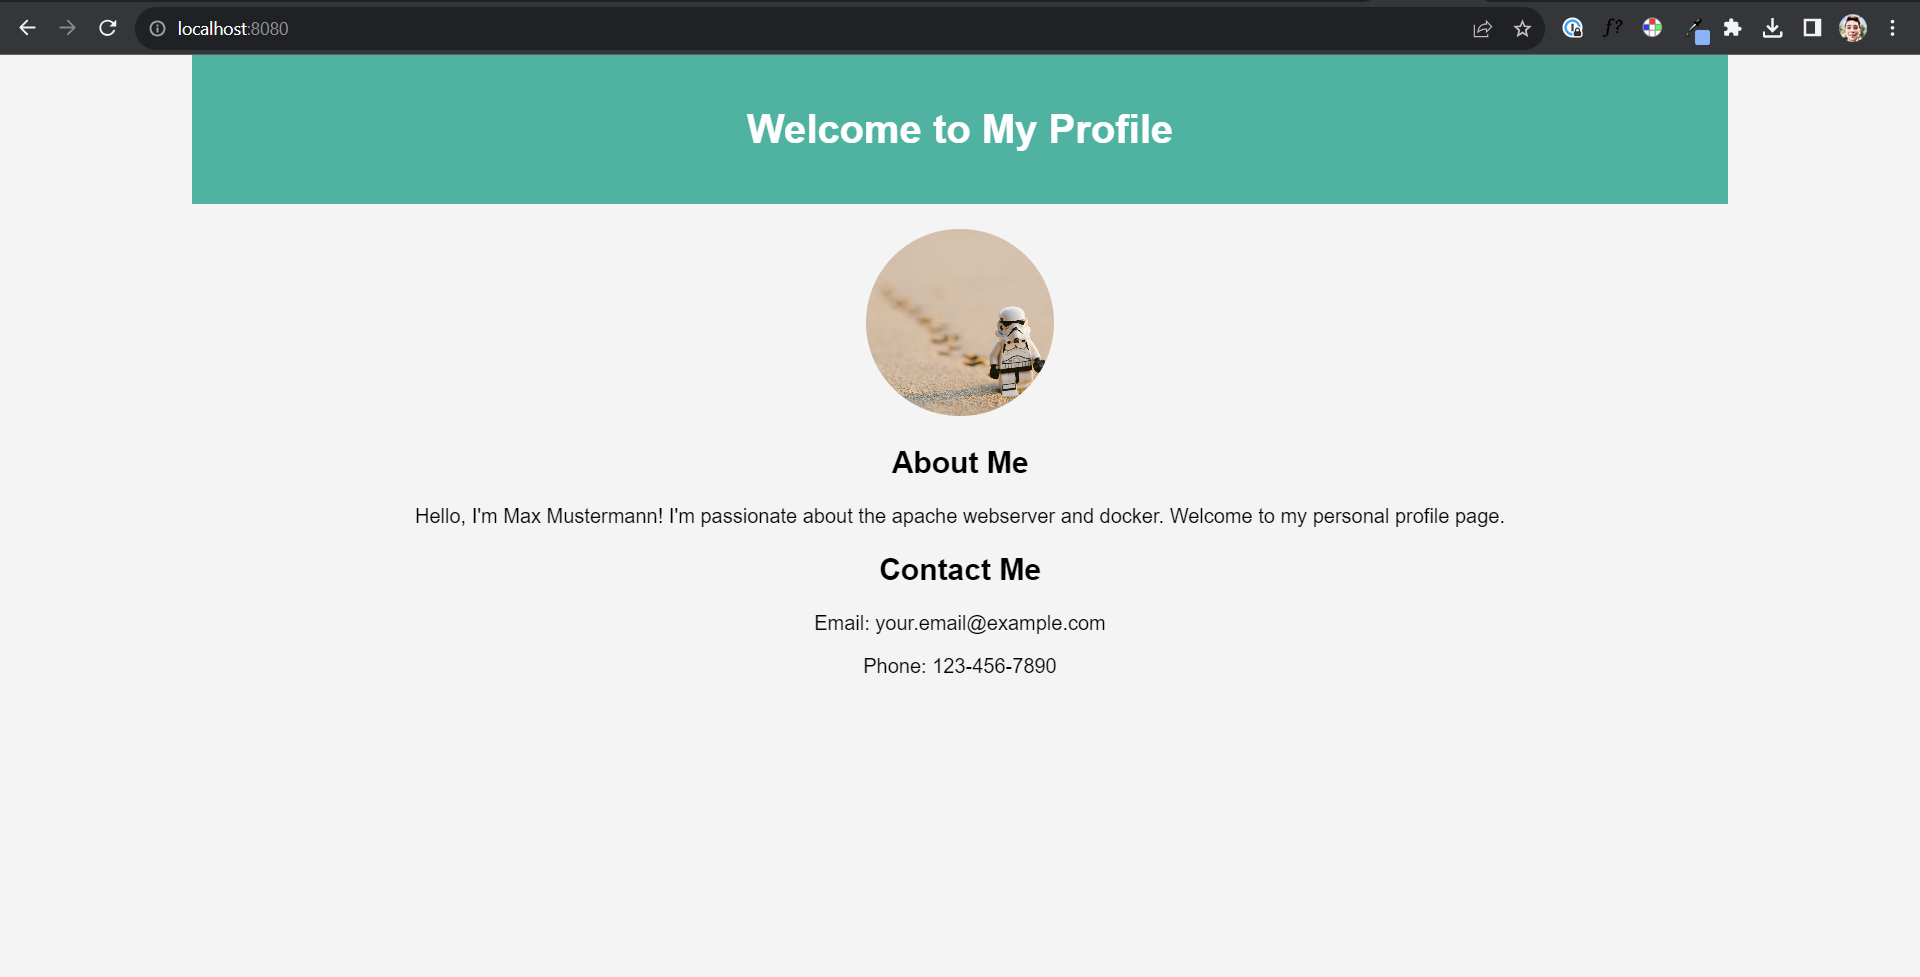
\includegraphics[width=15cm,height=14cm,keepaspectratio]{./images/screen}
        \caption{Die geladene Website}
        \label{fig:screen}
    \end{figure}


    \section{Aufgabe 2 - Python und Matplotlib}

    \subsection{Problem}
    In dieser Aufgabe soll mithilfe von Python und MatPlotLib eine Grafik einer Sinusfunktion ($f(x) = 10 * sin(x)^2$) erstellt werden.
    Daf"ur muss:
    \begin{enumerate}
        \item Python installiert werden
        \item Die Bibliotheken matplotlib und numpy installiert werden
        \item Das entsprechende Python-Script geschrieben werden
        \item Die generierte Bildatei in die Website eingebunden werden.
    \end{enumerate}

    \subsection{konkrete L"osung}

    \subsubsection{Bibliotheken}
    Nach der Installation von Python (hier apt install python3) k"onnen die beiden Bibliotheken numpy und matplotlib installiert werden. Dies geschieht mit dem "pip" Befehl (dem Python Paketmanager)
    \begin{lstlisting}
        pip install numpy matplotlib
    \end{lstlisting}
    Um eine \textbf{requirements.txt} Datei zu erstellen, um die Projektabh"angigkeiten anzugeben kann der Befehl \textbf{pip freeze $>$ requirements.txt} verwendet werden.

    \subsubsection{Python-Script}
    Als n"achstes muss das entsprechende Python-Skript (hier main.py) erstellt werden.

    Zun"achst m"ussen die Bibliotheken (hier mit Alias) importiert werden:
    \begin{lstlisting}[language=Python]
        import matplotlib.pyplot as plt
        import numpy as np
    \end{lstlisting}
    Danach kann die eigentliche Funktion definiert werden.
    \begin{lstlisting}[language=Python]
        def function(x):
            return 10 * np.sin(x) ** 2
    \end{lstlisting}
    Die Funktion wird hier von 0 bis 10 in 0.1er Schritten ausgewertet. Daf"ur k"onnen wir mit np.arangae ein Array aus Zahlen erstellen:
    \begin{lstlisting}[language=Python]
        values = np.arange(0, 10, 0.1)
    \end{lstlisting}
    Dies x-Werte k"onnen nun mithilfe der definierten Funktion function ausgewertet werden:
    \begin{lstlisting}[language=Python]
        y_values = function(values)
    \end{lstlisting}

    Schließlich kann mithilfe von matplotlib die Grafik erstellt werden:
    \begin{lstlisting}[language=Python]
        plt.plot(values, y_values, label='f(x) = 10 * (sin(x))^2')
        plt.title('Graph of the function f(x): G_f')
        plt.xlabel('x')
        plt.ylabel('f(x)')
        plt.legend()
        plt.grid(True)
        plt.savefig('python_output.png')
    \end{lstlisting}
    \begin{enumerate}
        \item Plot erstellt den "Plot" mit den x und y Werten, sowie der Beschriftung der Funktion
        \item plt.title gibt der Grafik einen Titel
        \item plt.xlabel und plt.ylabel beschriften die Achsen
        \item plt.legend f"ugt eine Legende hinzu
        \item plt.grid(True) f"ugt ein Gitter (sprich ein "kariertes Koordinatensystem" )hinzu
        \item plt.savefig speichert die Grafik als Bild ab.
    \end{enumerate}

    \subsection{Tests}
    Danach sollte die Datei in ./output.png gespeichert werden. Wenn wir die Datei auf unsere Website einbinden, k"onnen wir theoretisch sogar direkt den entsprechenden Pfad angeben:
    \textbf{/var/www/html/eii/function.png}
    Somit wird immer die aktuelle Funktionsgrafik auf unserer Website eingebettet.


    \section{Resumee zur dieser "Ubungsaufgabe}
    Dauer f"ur
    \begin
    {itemize}
        \item Durchf"uhrung: 20min
        \item Dokumentation: 15min
    \end{itemize}


    \section{Anlagen}
    \begin{figure}[h]
        \centering
        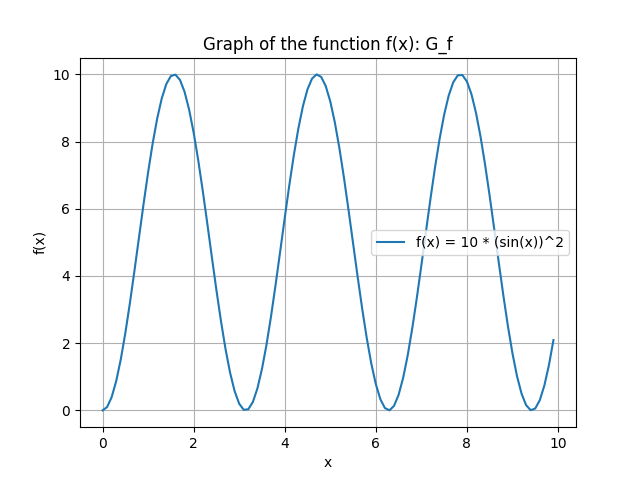
\includegraphics[width=15cm,height=14cm,keepaspectratio]{./images/function}
        \caption{Die generierte Grafik}
        \label{fig:function}
    \end{figure}

    \begin{figure}[h]
        \centering
        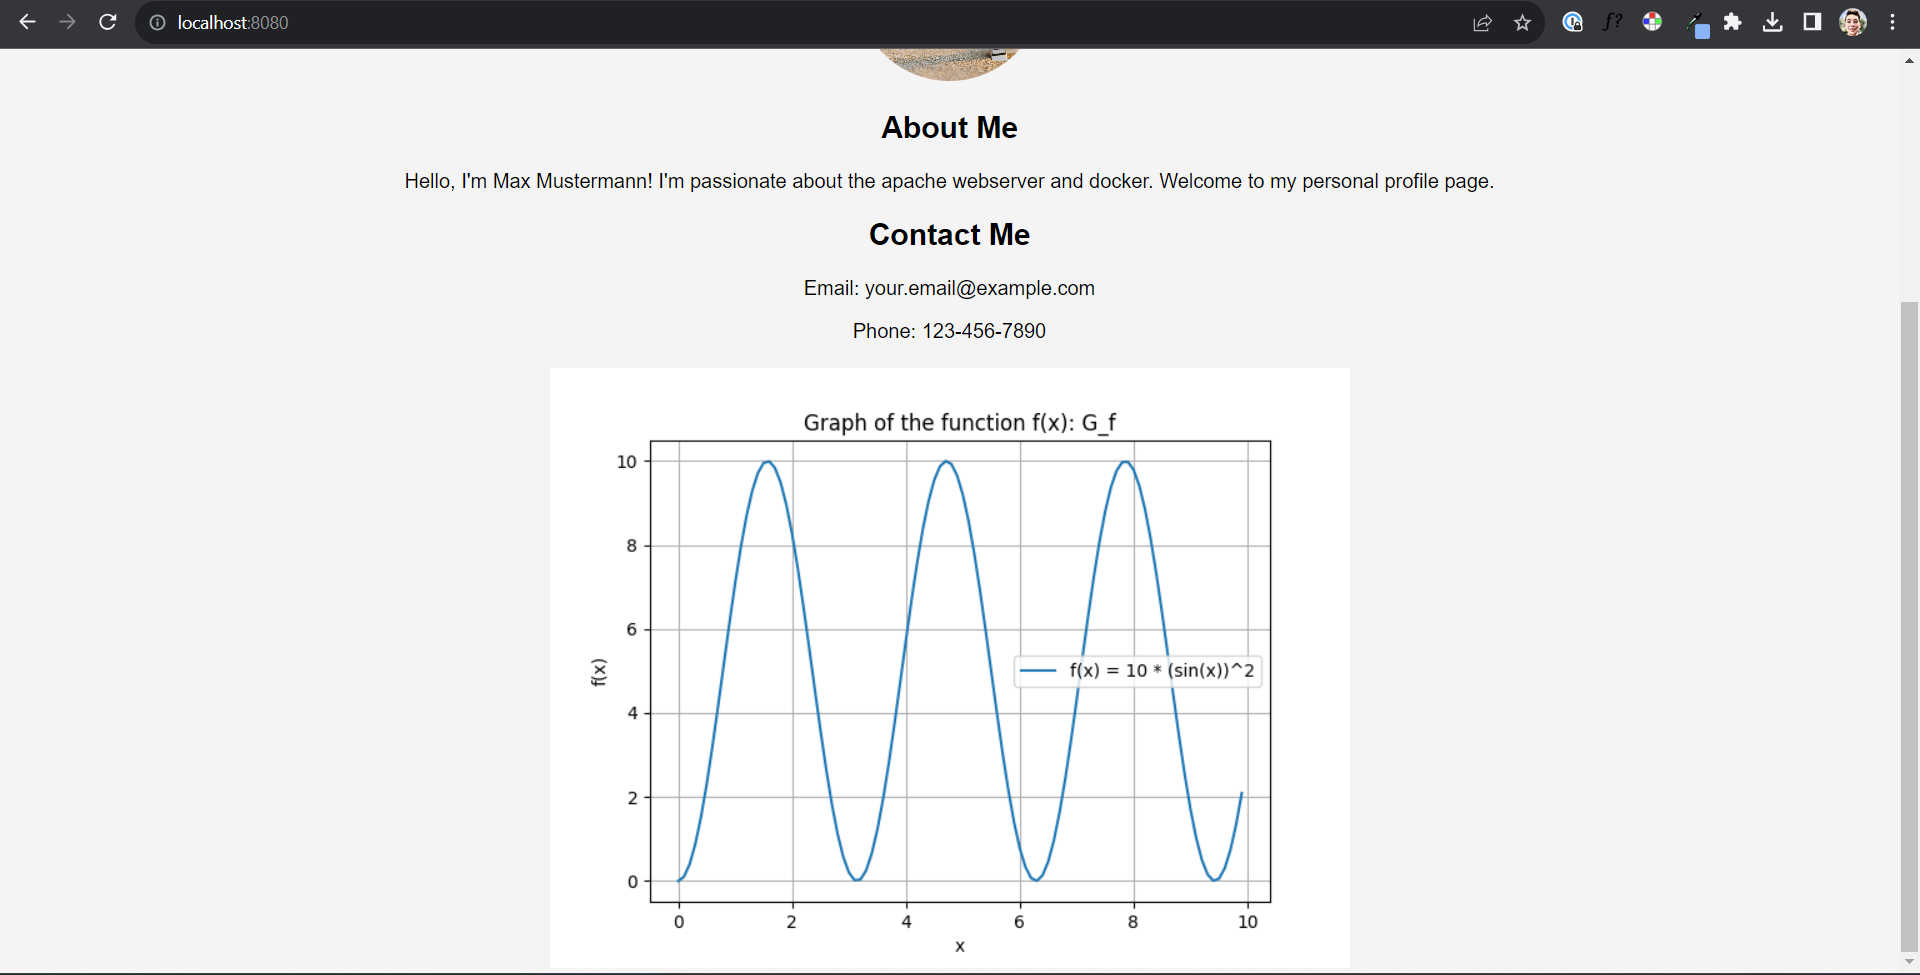
\includegraphics[width=15cm,height=14cm,keepaspectratio]{./images/screen2}
        \caption{Die Grafik auf der Website}
        \label{fig:screen2}
    \end{figure}


\end{document}
